\documentclass{article}\usepackage[]{graphicx}\usepackage[]{color}
%% maxwidth is the original width if it is less than linewidth
%% otherwise use linewidth (to make sure the graphics do not exceed the margin)
\makeatletter
\def\maxwidth{ %
  \ifdim\Gin@nat@width>\linewidth
    \linewidth
  \else
    \Gin@nat@width
  \fi
}
\makeatother

\definecolor{fgcolor}{rgb}{0.345, 0.345, 0.345}
\newcommand{\hlnum}[1]{\textcolor[rgb]{0.686,0.059,0.569}{#1}}%
\newcommand{\hlstr}[1]{\textcolor[rgb]{0.192,0.494,0.8}{#1}}%
\newcommand{\hlcom}[1]{\textcolor[rgb]{0.678,0.584,0.686}{\textit{#1}}}%
\newcommand{\hlopt}[1]{\textcolor[rgb]{0,0,0}{#1}}%
\newcommand{\hlstd}[1]{\textcolor[rgb]{0.345,0.345,0.345}{#1}}%
\newcommand{\hlkwa}[1]{\textcolor[rgb]{0.161,0.373,0.58}{\textbf{#1}}}%
\newcommand{\hlkwb}[1]{\textcolor[rgb]{0.69,0.353,0.396}{#1}}%
\newcommand{\hlkwc}[1]{\textcolor[rgb]{0.333,0.667,0.333}{#1}}%
\newcommand{\hlkwd}[1]{\textcolor[rgb]{0.737,0.353,0.396}{\textbf{#1}}}%

\usepackage{framed}
\makeatletter
\newenvironment{kframe}{%
 \def\at@end@of@kframe{}%
 \ifinner\ifhmode%
  \def\at@end@of@kframe{\end{minipage}}%
  \begin{minipage}{\columnwidth}%
 \fi\fi%
 \def\FrameCommand##1{\hskip\@totalleftmargin \hskip-\fboxsep
 \colorbox{shadecolor}{##1}\hskip-\fboxsep
     % There is no \\@totalrightmargin, so:
     \hskip-\linewidth \hskip-\@totalleftmargin \hskip\columnwidth}%
 \MakeFramed {\advance\hsize-\width
   \@totalleftmargin\z@ \linewidth\hsize
   \@setminipage}}%
 {\par\unskip\endMakeFramed%
 \at@end@of@kframe}
\makeatother

\definecolor{shadecolor}{rgb}{.97, .97, .97}
\definecolor{messagecolor}{rgb}{0, 0, 0}
\definecolor{warningcolor}{rgb}{1, 0, 1}
\definecolor{errorcolor}{rgb}{1, 0, 0}
\newenvironment{knitrout}{}{} % an empty environment to be redefined in TeX

\usepackage{alltt}
\usepackage{amscd, amssymb, amsmath, verbatim, setspace}
\usepackage[left=1.0in, right=1.0in, top=1.0in, bottom=1.0in]{geometry}
\usepackage{mathrsfs}
\usepackage{listings}


\IfFileExists{upquote.sty}{\usepackage{upquote}}{}
\begin{document}
\begin{flushright}
Arif Ali\\
Analytics 512 Statistical Learning\\
May 12, 2016\\
\end{flushright}

\begin{center}
\LARGE\textbf{Final Exam take home portion}
  \end{center}
\begin{knitrout}
\definecolor{shadecolor}{rgb}{0.969, 0.969, 0.969}\color{fgcolor}\begin{kframe}
\begin{alltt}
\hlkwd{library}\hlstd{(}\hlstr{"mlbench"}\hlstd{)}
\hlkwd{data}\hlstd{(Ozone)}
\hlstd{Ozone} \hlkwb{=} \hlkwd{as.data.frame}\hlstd{(}\hlkwd{mapply}\hlstd{(as.numeric, Ozone))}
\end{alltt}
\end{kframe}
\end{knitrout}
\section*{Exercise 1}
\begin{knitrout}
\definecolor{shadecolor}{rgb}{0.969, 0.969, 0.969}\color{fgcolor}\begin{kframe}
\begin{alltt}
\hlkwd{set.seed}\hlstd{(}\hlnum{1933}\hlstd{)}
\hlkwd{names}\hlstd{(Ozone)} \hlkwb{<-} \hlkwd{c}\hlstd{(}\hlstr{"mo"}\hlstd{,}\hlstr{"day"}\hlstd{,}\hlstr{"wday"}\hlstd{,}\hlstr{"maxoz"}\hlstd{,}\hlstr{"pressh"}\hlstd{,}\hlstr{"wind"}\hlstd{,}\hlstr{"hum"}\hlstd{,}
                  \hlstr{"temp1"}\hlstd{,}\hlstr{"temp2"}\hlstd{,}\hlstr{"inverh"}\hlstd{,}\hlstr{"pressg"}\hlstd{,}\hlstr{"invert"}\hlstd{,}\hlstr{"vis"}\hlstd{)}
\hlstd{Ozone}\hlopt{$}\hlstd{time} \hlkwb{=} \hlnum{1}\hlopt{:}\hlnum{366}
\hlstd{Ozone} \hlkwb{=} \hlstd{Ozone[}\hlopt{!}\hlkwd{is.na}\hlstd{(Ozone}\hlopt{$}\hlstd{maxoz),]}
\hlstd{train} \hlkwb{=} \hlkwd{sample}\hlstd{(}\hlkwd{nrow}\hlstd{(Ozone),} \hlkwd{nrow}\hlstd{(Ozone)}\hlopt{*}\hlnum{.70}\hlstd{)}
\hlstd{Ozone_train} \hlkwb{=} \hlstd{Ozone[train,]}
\end{alltt}
\end{kframe}
\end{knitrout}
Any observations were maxoz is na is dropped because, if there is no response variable, then the observation is not useful because there is no way to benchmark the values.
\section*{Exercise 2}
\begin{knitrout}
\definecolor{shadecolor}{rgb}{0.969, 0.969, 0.969}\color{fgcolor}\begin{kframe}
\begin{alltt}
\hlkwd{library}\hlstd{(boot)}
\hlstd{poly.cv.error} \hlkwb{=} \hlkwd{c}\hlstd{()}
\hlstd{d} \hlkwb{=} \hlnum{1}\hlopt{:}\hlnum{10}
\hlkwa{for}\hlstd{(i} \hlkwa{in} \hlstd{d)\{}
  \hlstd{ozone_pm} \hlkwb{=} \hlkwd{glm}\hlstd{(maxoz}\hlopt{~}\hlkwd{poly}\hlstd{(time,i),} \hlkwc{data} \hlstd{= Ozone_train)}
  \hlstd{poly.cv.error[i]} \hlkwb{=} \hlkwd{cv.glm}\hlstd{(Ozone_train, ozone_pm,} \hlkwc{K} \hlstd{=} \hlnum{10}\hlstd{)}\hlopt{$}\hlstd{delta[}\hlnum{2}\hlstd{]}
\hlstd{\}}
\hlkwd{plot}\hlstd{(d,poly.cv.error,}\hlkwc{type}\hlstd{=}\hlstr{"b"}\hlstd{)}
\end{alltt}
\end{kframe}
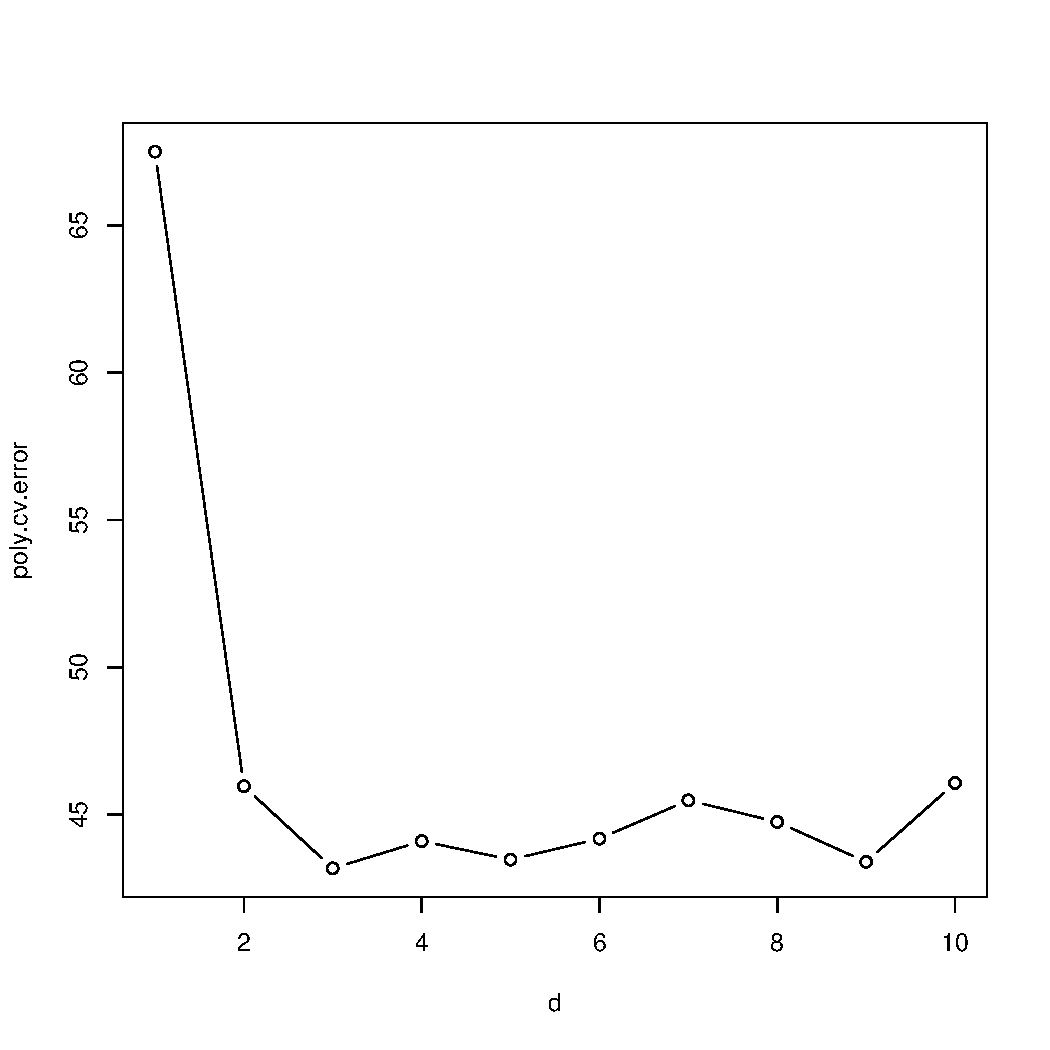
\includegraphics[width=0.40\linewidth]{figure/unnamed-chunk-4-1} 
\begin{kframe}\begin{alltt}
\hlstd{ozone_pm} \hlkwb{=} \hlkwd{lm}\hlstd{(maxoz}\hlopt{~}\hlkwd{poly}\hlstd{(time,d[poly.cv.error} \hlopt{==} \hlkwd{min}\hlstd{(poly.cv.error)]),} \hlkwc{data} \hlstd{= Ozone_train)}
\hlstd{RSS} \hlkwb{=} \hlkwd{sum}\hlstd{((}\hlkwd{predict}\hlstd{(ozone_pm, Ozone[}\hlopt{-}\hlstd{train,])}\hlopt{-}\hlstd{Ozone[}\hlopt{-}\hlstd{train,}\hlstr{"maxoz"}\hlstd{])}\hlopt{^}\hlnum{2}\hlstd{)}
\hlstd{RSE} \hlkwb{=} \hlkwd{sqrt}\hlstd{(RSS}\hlopt{/}\hlstd{(}\hlkwd{nrow}\hlstd{(Ozone[}\hlopt{-}\hlstd{train,])))}
\end{alltt}
\end{kframe}
\end{knitrout}
Cross Validation identified 7 as the degree of polynomial best suited for predicting Max Ozone. The test Residual Standard Error is 6.7276186.

\section*{Exercise 3}
\begin{knitrout}
\definecolor{shadecolor}{rgb}{0.969, 0.969, 0.969}\color{fgcolor}\begin{kframe}
\begin{alltt}
\hlkwd{library}\hlstd{(splines)}
\hlstd{RSE} \hlkwb{=} \hlnum{2}\hlopt{:}\hlnum{40}
\hlkwa{for}\hlstd{(i} \hlkwa{in} \hlnum{2}\hlopt{:}\hlnum{40}\hlstd{)\{}

  \hlstd{ozone_smoothing.splines} \hlkwb{=} \hlkwd{smooth.spline}\hlstd{(Ozone_train}\hlopt{$}\hlstd{time,}
                                          \hlstd{Ozone_train}\hlopt{$}\hlstd{maxoz,} \hlkwc{df} \hlstd{= i)}
   \hlstd{RSS} \hlkwb{=} \hlkwd{sum}\hlstd{((}\hlkwd{predict}\hlstd{(ozone_smoothing.splines,}
                     \hlstd{Ozone[}\hlopt{-}\hlstd{train,}\hlstr{"time"}\hlstd{])}\hlopt{$}\hlstd{y}\hlopt{-}\hlstd{Ozone[}\hlopt{-}\hlstd{train,}\hlstr{"maxoz"}\hlstd{])}\hlopt{^}\hlnum{2}\hlstd{)}
   \hlstd{RSE[i}\hlopt{-}\hlnum{1}\hlstd{]} \hlkwb{=} \hlkwd{sqrt}\hlstd{(RSS}\hlopt{/}\hlstd{(}\hlkwd{nrow}\hlstd{(Ozone[}\hlopt{-}\hlstd{train,])))}
\hlstd{\}}
\hlkwd{plot}\hlstd{(}\hlnum{2}\hlopt{:}\hlnum{40}\hlstd{, RSE,} \hlkwc{xlab} \hlstd{=} \hlstr{"degrees of freedom"}\hlstd{,} \hlkwc{type} \hlstd{=} \hlstr{"b"}\hlstd{)}


\hlkwd{points}\hlstd{((}\hlkwd{which.min}\hlstd{(RSE)}\hlopt{+}\hlnum{1}\hlstd{),}
       \hlstd{RSE[}\hlkwd{which.min}\hlstd{(RSE)],}
       \hlkwc{col}\hlstd{=}\hlstr{"red"}\hlstd{,}\hlkwc{cex}\hlstd{=}\hlnum{2}\hlstd{,}\hlkwc{pch}\hlstd{=}\hlnum{20}\hlstd{)}
\end{alltt}
\end{kframe}
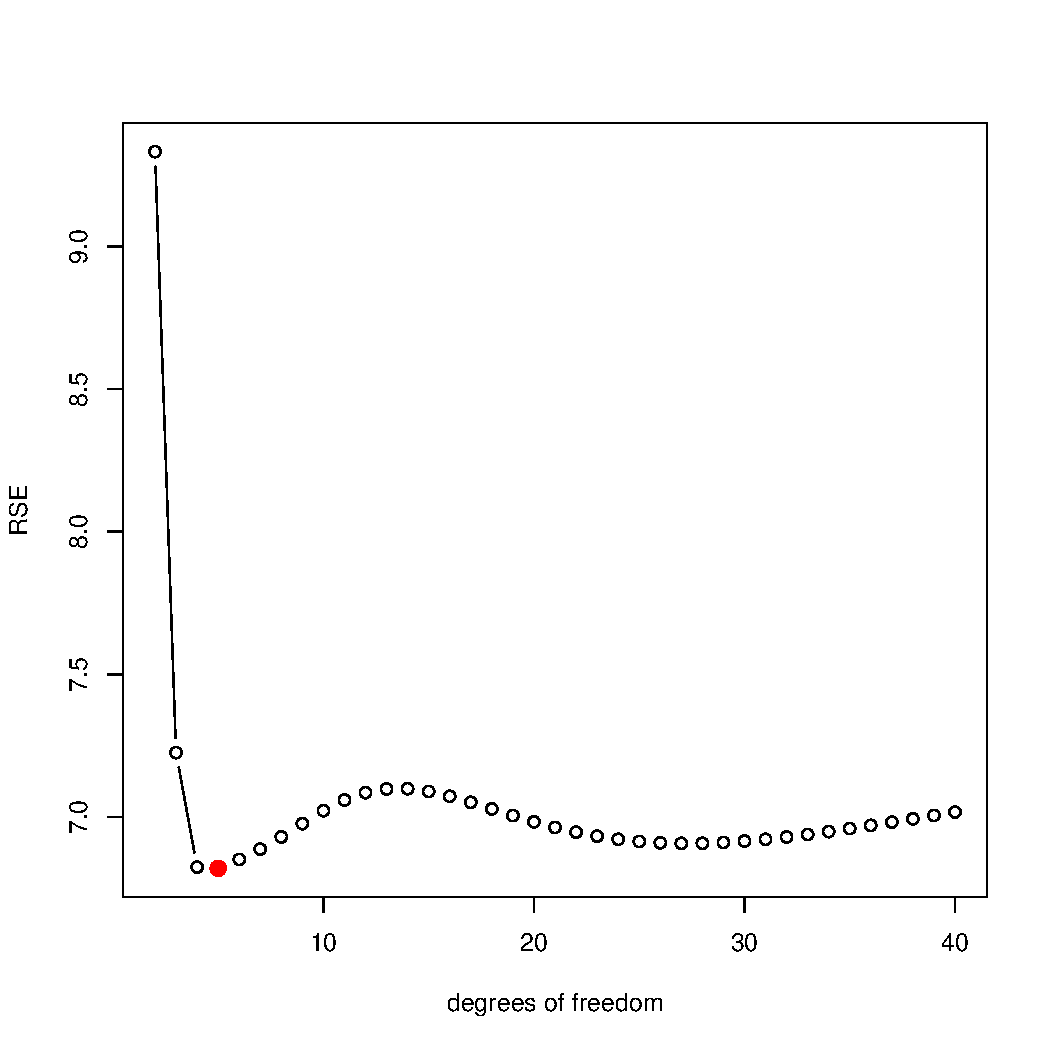
\includegraphics[width=0.40\linewidth]{figure/unnamed-chunk-5-1} 

\end{knitrout}
Using the Validation set approach, a smooth spline with 40 degrees of freedom is best suited for predicting Max Ozone. The test Residual Standard Error at 40 degrees of freedom is 5.7442268. It's interesting to see such a sudden drop in RSE from 2 to 40 degrees of freedom, but after-wards, a wave like structure occur. I wondering if more than 40 degrees of freedom were explored, if the wave would just continue.
\section*{Exercise 4}
\begin{knitrout}
\definecolor{shadecolor}{rgb}{0.969, 0.969, 0.969}\color{fgcolor}\begin{kframe}
\begin{alltt}
\hlkwd{library}\hlstd{(leaps)}
\hlstd{ozone_best_subset} \hlkwb{=} \hlkwd{regsubsets}\hlstd{(maxoz}\hlopt{~}\hlstd{.,}\hlkwd{na.omit}\hlstd{(Ozone_train[,}\hlkwd{c}\hlstd{(}\hlstr{"maxoz"}\hlstd{,}\hlstr{"pressh"}\hlstd{,}\hlstr{"wind"}\hlstd{,}\hlstr{"hum"}\hlstd{,}
                  \hlstr{"temp1"}\hlstd{,}\hlstr{"temp2"}\hlstd{,}\hlstr{"inverh"}\hlstd{,}\hlstr{"pressg"}\hlstd{,}\hlstr{"invert"}\hlstd{,}\hlstr{"vis"}\hlstd{)]))}
\hlkwd{plot}\hlstd{(}\hlkwd{summary}\hlstd{(ozone_best_subset)}\hlopt{$}\hlstd{bic ,}
     \hlkwc{xlab}\hlstd{=}\hlstr{"Number of Variables "}\hlstd{,}\hlkwc{ylab}\hlstd{=}\hlstr{"BIC"}\hlstd{,} \hlkwc{type}\hlstd{=}\hlstr{'l'}\hlstd{)}
\hlkwd{points}\hlstd{(}\hlkwd{which.min}\hlstd{(}\hlkwd{summary}\hlstd{(ozone_best_subset)}\hlopt{$}\hlstd{bic),}
       \hlkwd{summary}\hlstd{(ozone_best_subset)}\hlopt{$}\hlstd{bic[}\hlkwd{which.min}\hlstd{(}\hlkwd{summary}\hlstd{(ozone_best_subset)}\hlopt{$}\hlstd{bic)],}
       \hlkwc{col}\hlstd{=}\hlstr{"red"}\hlstd{,}\hlkwc{cex}\hlstd{=}\hlnum{2}\hlstd{,}\hlkwc{pch}\hlstd{=}\hlnum{20}\hlstd{)}
\end{alltt}
\end{kframe}
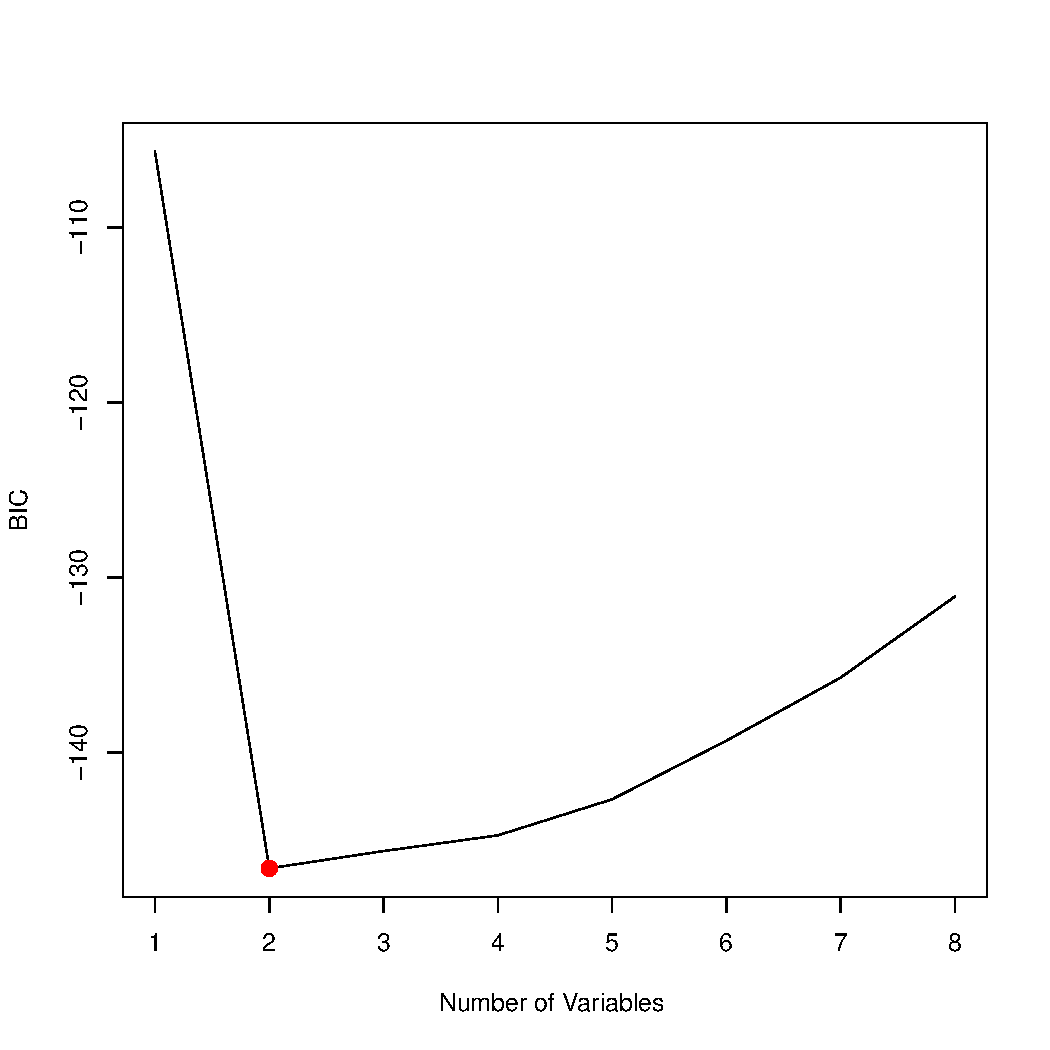
\includegraphics[width=0.40\linewidth]{figure/unnamed-chunk-6-1} 
\begin{kframe}\begin{alltt}
\hlstd{model} \hlkwb{=} \hlkwd{coef}\hlstd{(ozone_best_subset ,}\hlkwd{which.min}\hlstd{(}\hlkwd{summary}\hlstd{(ozone_best_subset)}\hlopt{$}\hlstd{bic))[}\hlopt{-}\hlnum{1}\hlstd{]}


\hlstd{best_oz_model} \hlkwb{=} \hlkwd{glm}\hlstd{(maxoz}\hlopt{~}\hlstd{.,} \hlkwd{na.omit}\hlstd{(Ozone_train[,} \hlkwd{c}\hlstd{(}\hlnum{4}\hlstd{,} \hlkwd{which}\hlstd{(}\hlkwd{names}\hlstd{(Ozone)} \hlopt \hlkwd{names}\hlstd{(model)))]),} \hlkwc{family} \hlstd{=} \hlstr{"gaussian"}\hlstd{)}

\hlstd{Ozone_test_na_omit} \hlkwb{=} \hlkwd{na.omit}\hlstd{(Ozone[}\hlopt{-}\hlstd{train,} \hlkwd{which}\hlstd{(}\hlkwd{names}\hlstd{(Ozone)} \hlopt \hlkwd{names}\hlstd{(model))])}

\hlstd{RSS} \hlkwb{=} \hlkwd{sum}\hlstd{((}\hlkwd{predict}\hlstd{(best_oz_model, Ozone_test_na_omit)}\hlopt{-}\hlstd{Ozone_test_na_omit[}\hlopt{-}\hlstd{train,}\hlnum{4}\hlstd{])}\hlopt{^}\hlnum{2}\hlstd{)}
\hlstd{RSE} \hlkwb{=} \hlkwd{sqrt}\hlstd{(RSS}\hlopt{/}\hlstd{(}\hlkwd{nrow}\hlstd{(Ozone[}\hlopt{-}\hlstd{train,])))}
\end{alltt}
\end{kframe}
\end{knitrout}
In order to attempt the best subset selection, the test and training observations' response and predictive variables cannot be NA, so na.omit needed to be applied on the datasets. Based in the plot, the subset with the lowest BIC is at 2 Best subset selection identified a model with the coefficients: hum,temp2 as the best performing model based on BIC. The model was then used to create a glm object, with equivalent coefficients: 0.1201742, 0.4491926 with a test RSE of 0
\section*{Exercise 5}
\begin{knitrout}
\definecolor{shadecolor}{rgb}{0.969, 0.969, 0.969}\color{fgcolor}\begin{kframe}
\begin{alltt}
\hlkwd{library}\hlstd{(glmnet)}
\end{alltt}


{\ttfamily\noindent\itshape\color{messagecolor}{\#\# Loading required package: Matrix\\\#\# Loading required package: foreach\\\#\# Loaded glmnet 2.0-2}}\begin{alltt}
\hlstd{grid} \hlkwb{=} \hlnum{10}\hlopt{^}\hlkwd{seq}\hlstd{(}\hlnum{10}\hlstd{,}\hlopt{-}\hlnum{2}\hlstd{,}\hlkwc{length}\hlstd{=}\hlnum{100}\hlstd{)}
\hlstd{x} \hlkwb{=} \hlkwd{model.matrix}\hlstd{(maxoz}\hlopt{~}\hlstd{.,}\hlkwd{na.omit}\hlstd{(Ozone_train))[,}\hlopt{-}\hlnum{1}\hlstd{]}
\hlstd{y} \hlkwb{=} \hlkwd{na.omit}\hlstd{(Ozone_train)}\hlopt{$}\hlstd{maxoz}
\hlstd{Ozone_lasso} \hlkwb{=} \hlkwd{glmnet}\hlstd{(x, y,} \hlkwc{alpha} \hlstd{=} \hlnum{1}\hlstd{,} \hlkwc{lambda} \hlstd{= grid)}
\hlstd{cv.out}\hlkwb{=}\hlkwd{cv.glmnet}\hlstd{(x,y,}\hlkwc{alpha}\hlstd{=}\hlnum{1}\hlstd{)}
\hlkwd{plot}\hlstd{(cv.out)}
\end{alltt}
\end{kframe}
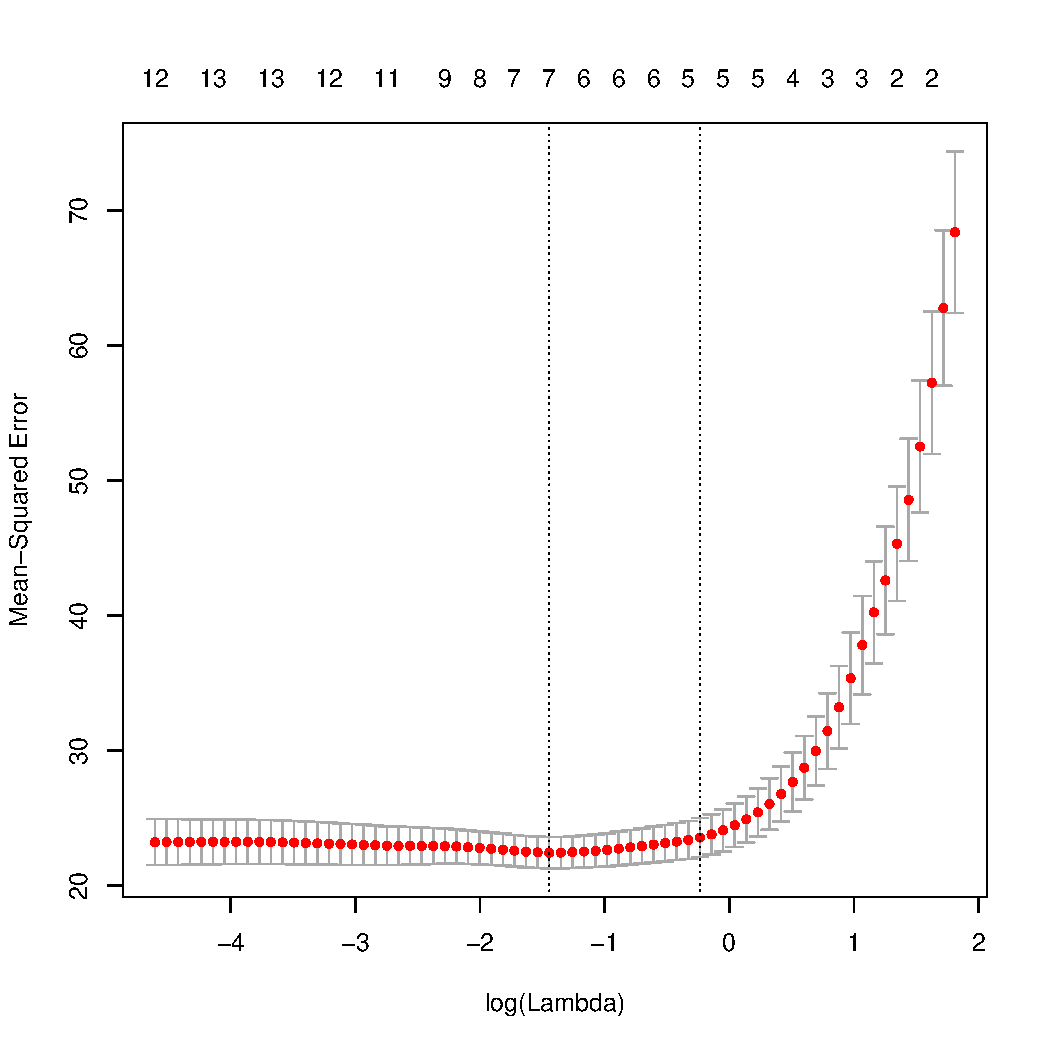
\includegraphics[width=0.40\linewidth]{figure/unnamed-chunk-7-1} 
\begin{kframe}\begin{alltt}
\hlstd{bestlam}\hlkwb{=}\hlstd{cv.out}\hlopt{$}\hlstd{lambda.min}


\hlstd{RSS} \hlkwb{=} \hlkwd{sum}\hlstd{((}\hlkwd{predict}\hlstd{(Ozone_lasso,}\hlkwc{s}\hlstd{=bestlam,}
                              \hlkwc{newx}\hlstd{=}\hlkwd{model.matrix}\hlstd{(maxoz}\hlopt{~}\hlstd{.,}\hlkwd{na.omit}\hlstd{(Ozone[}\hlopt{-}\hlstd{train,]))[,}\hlopt{-}\hlnum{1}\hlstd{]}
                   \hlstd{)}\hlopt{-}\hlkwd{na.omit}\hlstd{(Ozone[}\hlopt{-}\hlstd{train,])}\hlopt{$}\hlstd{maxoz)}\hlopt{^}\hlnum{2}\hlstd{)}
\hlstd{RSE} \hlkwb{=} \hlkwd{sqrt}\hlstd{(RSS}\hlopt{/}\hlstd{(}\hlkwd{nrow}\hlstd{(Ozone[}\hlopt{-}\hlstd{train,])))}

\hlstd{out}\hlkwb{=}\hlkwd{glmnet}\hlstd{(x,y,}\hlkwc{alpha}\hlstd{=}\hlnum{1}\hlstd{,}\hlkwc{lambda}\hlstd{=grid)}
\hlstd{lasso.coef}\hlkwb{=}\hlkwd{predict}\hlstd{(out,}\hlkwc{type}\hlstd{=}\hlstr{"coefficients"}\hlstd{,}\hlkwc{s}\hlstd{=bestlam)}
\end{alltt}
\end{kframe}
\end{knitrout}
The best parameter identified was $\lambda = 0.2348047$ after applying cross validation and using the lambda that obtained the lowest cross validation error. The coefficients, after applying the L1 penalty, were mo, day, hum, temp1, temp2, inverh, vis. The residual squared error was 3.5200735. The result performs better than the best subset selection based on the residual squared error, which is interesting and could indicate that solely looking at the BIC for best subset is not the best strategy.   
\section*{Exercise 6}
\subsection*{bagging}
\begin{knitrout}
\definecolor{shadecolor}{rgb}{0.969, 0.969, 0.969}\color{fgcolor}\begin{kframe}
\begin{alltt}
\hlkwd{library}\hlstd{(randomForest)}
\end{alltt}


{\ttfamily\noindent\itshape\color{messagecolor}{\#\# randomForest 4.6-12\\\#\# Type rfNews() to see new features/changes/bug fixes.}}\begin{alltt}
\hlstd{Ozone_clean_train} \hlkwb{=} \hlkwd{na.omit}\hlstd{(Ozone_train)}
\hlstd{Ozone_clean_test} \hlkwb{=} \hlkwd{na.omit}\hlstd{(Ozone[}\hlopt{-}\hlstd{train,])}

\hlstd{Ozone_bagging} \hlkwb{=} \hlkwd{randomForest}\hlstd{(maxoz}\hlopt{~}\hlstd{.,Ozone_clean_train,} \hlkwc{mtry} \hlstd{=} \hlkwd{ncol}\hlstd{(Ozone_train)}\hlopt{-}\hlnum{1}\hlstd{)}

\hlstd{RSS} \hlkwb{=} \hlkwd{sum}\hlstd{((}\hlkwd{predict}\hlstd{(Ozone_bagging ,}\hlkwc{newdata}\hlstd{=Ozone_clean_test)}\hlopt{-}\hlstd{(Ozone_clean_test}\hlopt{$}\hlstd{maxoz))}\hlopt{^}\hlnum{2}\hlstd{)}
\hlstd{RSE} \hlkwb{=} \hlkwd{sqrt}\hlstd{(RSS}\hlopt{/}\hlstd{(}\hlkwd{nrow}\hlstd{(Ozone[}\hlopt{-}\hlstd{train,])))}
\end{alltt}
\end{kframe}
\end{knitrout}
\subsection*{boosting}
\begin{knitrout}
\definecolor{shadecolor}{rgb}{0.969, 0.969, 0.969}\color{fgcolor}\begin{kframe}
\begin{alltt}
\hlkwd{library}\hlstd{(gbm)}
\end{alltt}


{\ttfamily\noindent\itshape\color{messagecolor}{\#\# Loading required package: survival\\\#\# \\\#\# Attaching package: 'survival'\\\#\# \\\#\# The following object is masked from 'package:boot':\\\#\# \\\#\#\ \ \ \  aml\\\#\# \\\#\# Loading required package: lattice\\\#\# \\\#\# Attaching package: 'lattice'\\\#\# \\\#\# The following object is masked from 'package:boot':\\\#\# \\\#\#\ \ \ \  melanoma\\\#\# \\\#\# Loading required package: parallel\\\#\# Loaded gbm 2.1.1}}\begin{alltt}
\hlstd{Ozone_boost}\hlkwb{=}\hlkwd{gbm}\hlstd{(maxoz}\hlopt{~}\hlstd{.,}\hlkwc{data}\hlstd{=Ozone[train,],}\hlkwc{distribution}\hlstd{=} \hlstr{"gaussian"}\hlstd{,} \hlkwc{n.trees}\hlstd{=}\hlnum{5000}\hlstd{,} \hlkwc{interaction.depth}\hlstd{=}\hlnum{4}\hlstd{)}


\hlstd{RSS} \hlkwb{=} \hlkwd{sum}\hlstd{((}\hlkwd{predict}\hlstd{(Ozone_boost,}\hlkwc{newdata}\hlstd{=Ozone[}\hlopt{-}\hlstd{train,],} \hlkwc{n.trees}\hlstd{=}\hlnum{5000}\hlstd{)}\hlopt{-}\hlstd{Ozone[}\hlopt{-}\hlstd{train,}\hlstr{"maxoz"}\hlstd{])}\hlopt{^}\hlnum{2}\hlstd{)}

\hlstd{RSE} \hlkwb{=} \hlkwd{sqrt}\hlstd{(RSS}\hlopt{/}\hlstd{(}\hlkwd{nrow}\hlstd{(Ozone[}\hlopt{-}\hlstd{train,])))}
\end{alltt}
\end{kframe}
\end{knitrout}
\subsection*{Random Forests}
\begin{knitrout}
\definecolor{shadecolor}{rgb}{0.969, 0.969, 0.969}\color{fgcolor}\begin{kframe}
\begin{alltt}
\hlstd{Ozone_rf} \hlkwb{=} \hlkwd{randomForest}\hlstd{(maxoz}\hlopt{~}\hlstd{.,Ozone_clean_train,} \hlkwc{mtry} \hlstd{= (}\hlkwd{ncol}\hlstd{(Ozone_train)}\hlopt{-}\hlnum{1}\hlstd{)}\hlopt{/}\hlnum{3}\hlstd{)}

\hlstd{RSS} \hlkwb{=} \hlkwd{sum}\hlstd{((}\hlkwd{predict}\hlstd{(Ozone_rf ,}\hlkwc{newdata}\hlstd{=Ozone_clean_test)}\hlopt{-}\hlstd{(Ozone_clean_test}\hlopt{$}\hlstd{maxoz))}\hlopt{^}\hlnum{2}\hlstd{)}
\hlstd{RSE} \hlkwb{=} \hlkwd{sqrt}\hlstd{(RSS}\hlopt{/}\hlstd{(}\hlkwd{nrow}\hlstd{(Ozone[}\hlopt{-}\hlstd{train,])))}
\end{alltt}
\end{kframe}
\end{knitrout}
\subsection*{Bonus}

\section*{Exercise 7}
\begin{knitrout}
\definecolor{shadecolor}{rgb}{0.969, 0.969, 0.969}\color{fgcolor}\begin{kframe}
\begin{alltt}
\hlstd{hepatitis} \hlkwb{<-} \hlkwd{read.csv}\hlstd{(}\hlstr{"hepatitis.data"}\hlstd{,} \hlkwc{header}\hlstd{=}\hlnum{FALSE}\hlstd{,} \hlkwc{na.strings} \hlstd{=} \hlstr{"?"}\hlstd{)}

\hlstd{training} \hlkwb{=} \hlkwd{sample}\hlstd{(}\hlkwd{nrow}\hlstd{(hepatitis),} \hlnum{105}\hlstd{)}

\hlstd{hep_train} \hlkwb{=} \hlstd{hepatitis[training,]}


\hlstd{hep_scale} \hlkwb{=} \hlkwd{scale}\hlstd{(hep_train)}
\hlstd{hc.out}\hlkwb{=}\hlkwd{hclust}\hlstd{(}\hlkwd{dist}\hlstd{(hep_scale),}  \hlkwc{method}\hlstd{=}\hlstr{"average"}\hlstd{)}
\hlstd{hc.clusters}\hlkwb{=}\hlkwd{cutree}\hlstd{(hc.out,}\hlnum{2}\hlstd{)}
\hlkwd{table}\hlstd{(hc.clusters,hep_train}\hlopt{$}\hlstd{V1)}
\end{alltt}
\begin{verbatim}
##            
## hc.clusters  1  2
##           1 16 87
##           2  2  0
\end{verbatim}
\begin{alltt}
\hlkwd{plot}\hlstd{(hc.out,} \hlkwc{labels}\hlstd{=hepatitis[training,}\hlnum{1}\hlstd{])}

\hlstd{hc.out}\hlkwb{=}\hlkwd{hclust}\hlstd{(}\hlkwd{dist}\hlstd{(hep_scale),}  \hlkwc{method}\hlstd{=}\hlstr{"complete"}\hlstd{)}
\hlstd{hc.clusters}\hlkwb{=}\hlkwd{cutree}\hlstd{(hc.out,}\hlnum{2}\hlstd{)}
\hlkwd{table}\hlstd{(hc.clusters,hep_train}\hlopt{$}\hlstd{V1)}
\end{alltt}
\begin{verbatim}
##            
## hc.clusters  1  2
##           1 16 85
##           2  2  2
\end{verbatim}
\begin{alltt}
\hlkwd{plot}\hlstd{(hc.out,} \hlkwc{labels}\hlstd{=hepatitis[training,}\hlnum{1}\hlstd{])}

\hlstd{hc.out}\hlkwb{=}\hlkwd{hclust}\hlstd{(}\hlkwd{dist}\hlstd{(hep_scale),}  \hlkwc{method}\hlstd{=}\hlstr{"single"}\hlstd{)}
\hlstd{hc.clusters}\hlkwb{=}\hlkwd{cutree}\hlstd{(hc.out,}\hlnum{2}\hlstd{)}
\hlkwd{table}\hlstd{(hc.clusters,hep_train}\hlopt{$}\hlstd{V1)}
\end{alltt}
\begin{verbatim}
##            
## hc.clusters  1  2
##           1 17 87
##           2  1  0
\end{verbatim}
\begin{alltt}
\hlkwd{plot}\hlstd{(hc.out,} \hlkwc{labels}\hlstd{=hepatitis[training,}\hlnum{1}\hlstd{])}
\end{alltt}
\end{kframe}
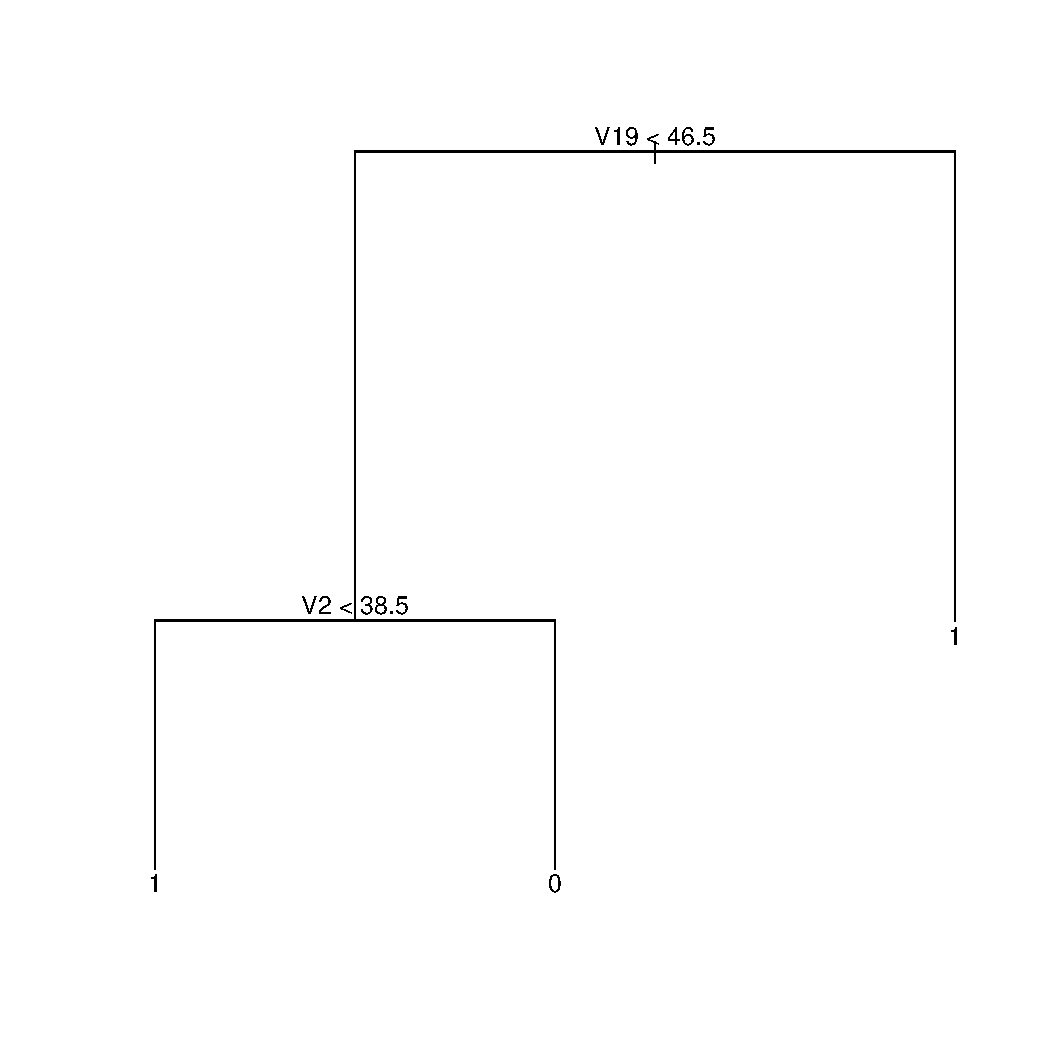
\includegraphics[width=0.40\linewidth]{figure/unnamed-chunk-12-1} 
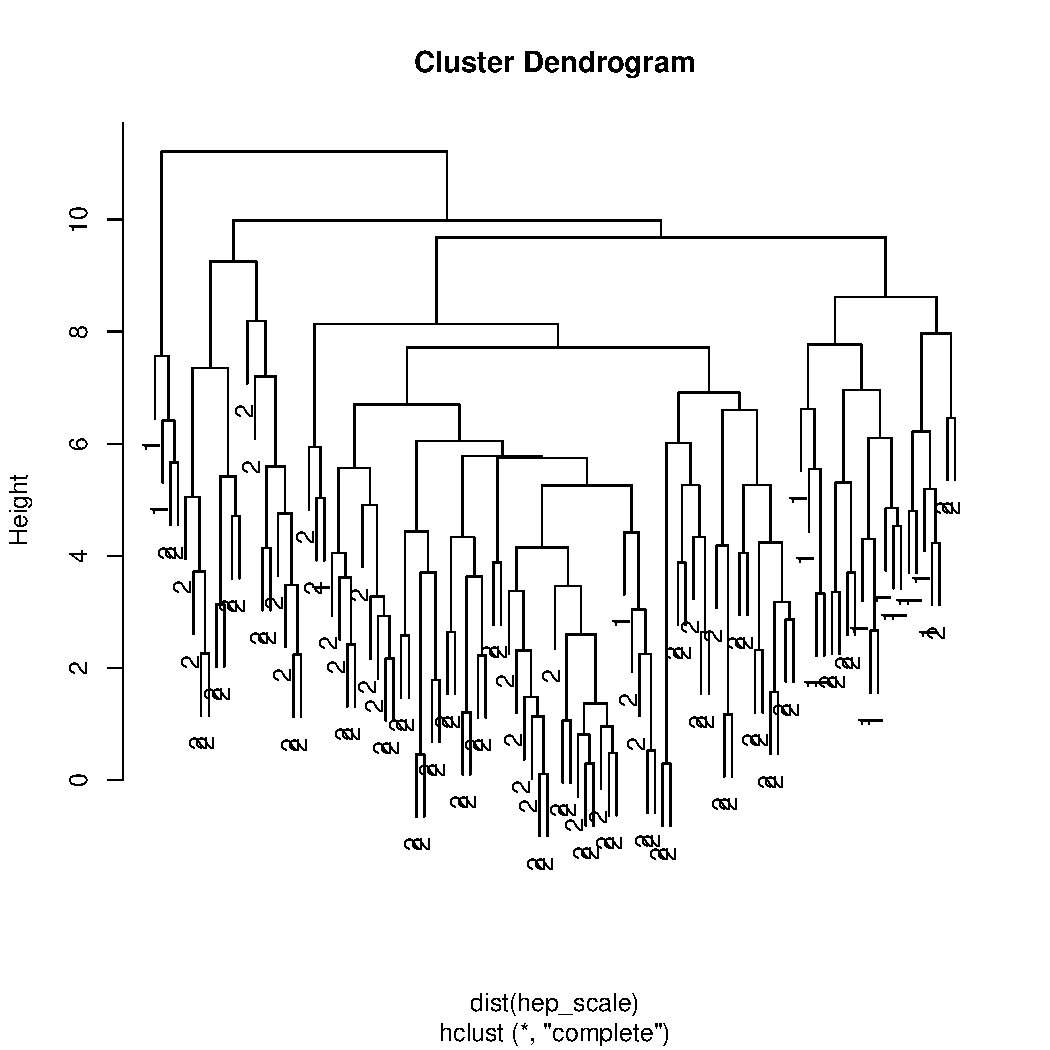
\includegraphics[width=0.40\linewidth]{figure/unnamed-chunk-12-2} 
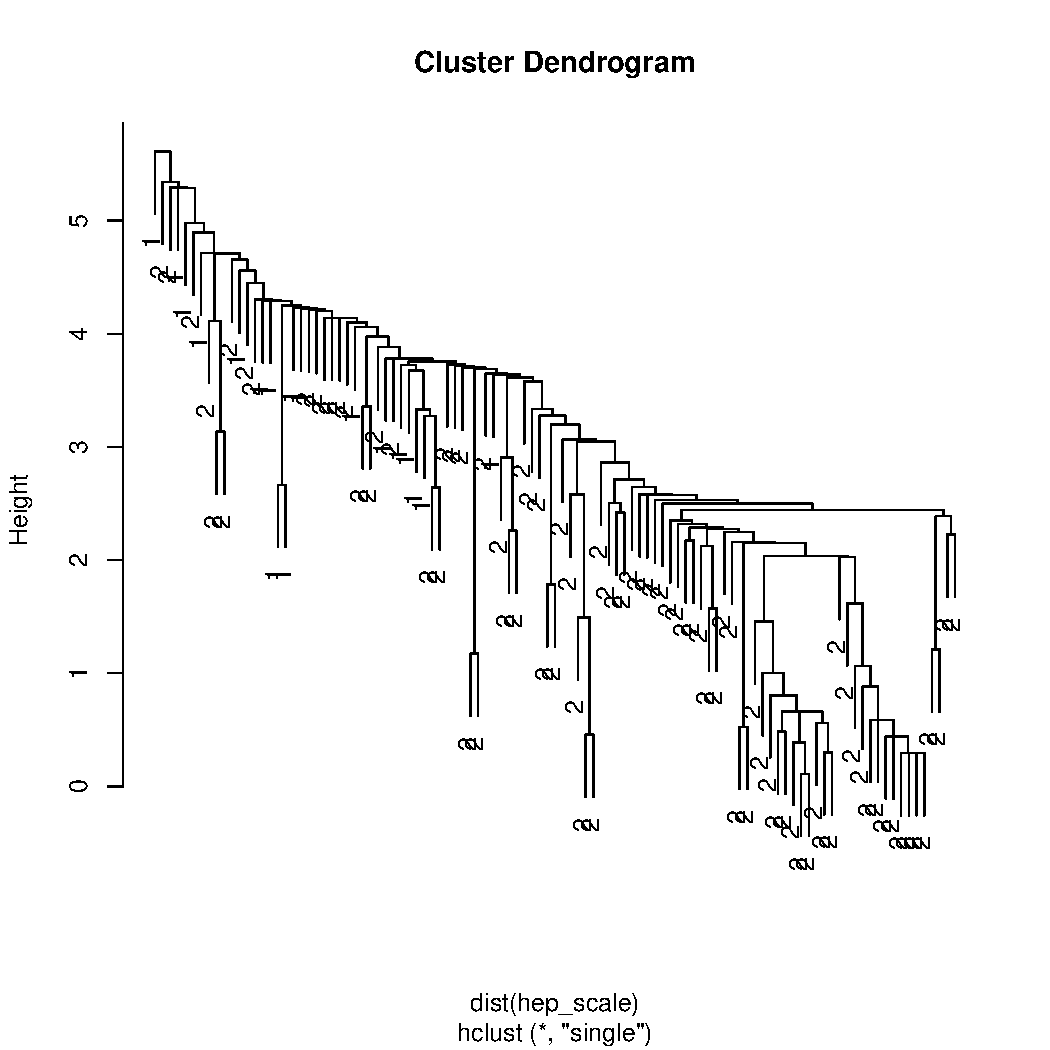
\includegraphics[width=0.40\linewidth]{figure/unnamed-chunk-12-3} 

\end{knitrout}

\begin{knitrout}
\definecolor{shadecolor}{rgb}{0.969, 0.969, 0.969}\color{fgcolor}\begin{kframe}
\begin{alltt}
\hlstd{hepatitis}\hlopt{$}\hlstd{V1} \hlkwb{=} \hlkwd{as.factor}\hlstd{(hepatitis}\hlopt{$}\hlstd{V1}\hlopt{-}\hlnum{1}\hlstd{)}
\hlstd{hep_train} \hlkwb{=} \hlstd{hepatitis[training,]}


\hlstd{hep_boost} \hlkwb{=} \hlkwd{gbm}\hlstd{(V1}\hlopt{~}\hlstd{.,}\hlkwc{data} \hlstd{= hep_train,} \hlkwc{distribution} \hlstd{=} \hlstr{"multinomial"}\hlstd{,} \hlkwc{n.trees}\hlstd{=}\hlnum{1000}\hlstd{)}
\hlstd{yhat.boost}\hlkwb{=}\hlkwd{as.data.frame}\hlstd{(}\hlkwd{predict}\hlstd{(hep_boost,}\hlkwc{newdata}\hlstd{=hepatitis[}\hlopt{-}\hlstd{training,],} \hlkwc{n.trees}\hlstd{=}\hlnum{1000}\hlstd{,}  \hlkwc{type} \hlstd{=} \hlstr{"response"}\hlstd{))}
\hlstd{boot_results} \hlkwb{=} \hlnum{1}\hlopt{:}\hlnum{50}
\hlstd{boot_results[yhat.boost[,}\hlnum{1}\hlstd{]}\hlopt{>}\hlstd{yhat.boost[,}\hlnum{2}\hlstd{]]}\hlkwb{=}\hlnum{0}
\hlstd{boot_results[yhat.boost[,}\hlnum{2}\hlstd{]}\hlopt{>}\hlstd{yhat.boost[,}\hlnum{1}\hlstd{]]}\hlkwb{=}\hlnum{1}

\hlkwd{mean}\hlstd{(boot_results} \hlopt{!=} \hlstd{hepatitis}\hlopt{$}\hlstd{V1[}\hlopt{-}\hlstd{training])}
\end{alltt}
\begin{verbatim}
## [1] 0.26
\end{verbatim}
\begin{alltt}
\hlkwd{table}\hlstd{(boot_results, hepatitis}\hlopt{$}\hlstd{V1[}\hlopt{-}\hlstd{training])}
\end{alltt}
\begin{verbatim}
##             
## boot_results  0  1
##            0  2  1
##            1 12 35
\end{verbatim}
\end{kframe}
\end{knitrout}

\begin{knitrout}
\definecolor{shadecolor}{rgb}{0.969, 0.969, 0.969}\color{fgcolor}\begin{kframe}
\begin{alltt}
\hlkwd{library}\hlstd{(tree)}
\hlstd{hep_tree} \hlkwb{=} \hlkwd{tree}\hlstd{(}\hlkwc{formula} \hlstd{= V1} \hlopt{~} \hlstd{.,} \hlkwc{data} \hlstd{= hep_train)}
\hlkwd{summary}\hlstd{(hep_tree)}
\end{alltt}
\begin{verbatim}
## 
## Classification tree:
## tree(formula = V1 ~ ., data = hep_train)
## Variables actually used in tree construction:
## [1] "V15" "V18" "V2" 
## Number of terminal nodes:  5 
## Residual mean deviance:  0.2529 = 12.14 / 48 
## Misclassification error rate: 0.0566 = 3 / 53
\end{verbatim}
\begin{alltt}
\hlkwd{plot}\hlstd{(hep_tree)}
\hlkwd{text}\hlstd{(hep_tree ,}\hlkwc{pretty} \hlstd{=}\hlnum{0}\hlstd{)}
\end{alltt}
\end{kframe}
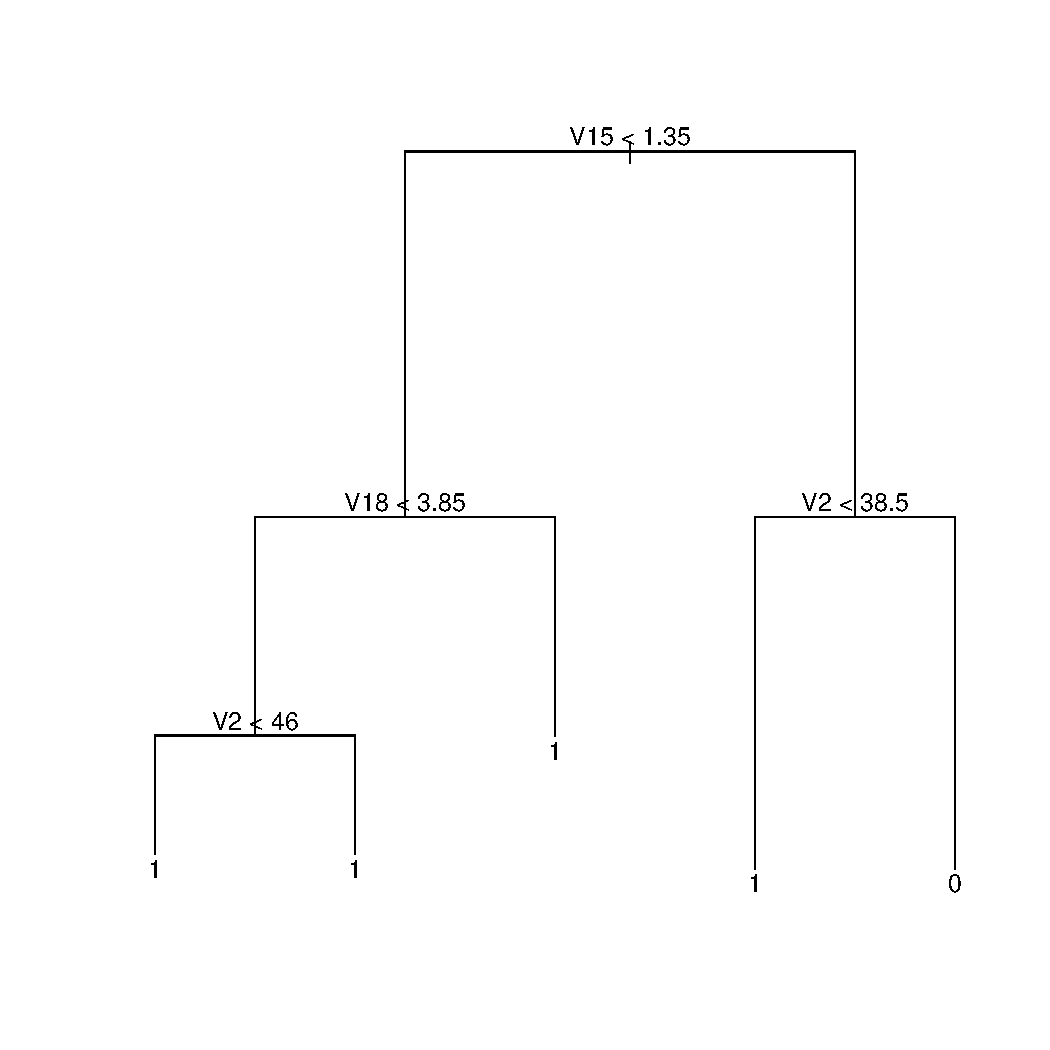
\includegraphics[width=0.40\linewidth]{figure/unnamed-chunk-14-1} 
\begin{kframe}\begin{alltt}
\hlstd{tree_pred} \hlkwb{=} \hlkwd{predict}\hlstd{(hep_tree, hepatitis[}\hlopt{-}\hlstd{training,],} \hlkwc{type} \hlstd{=} \hlstr{"class"}\hlstd{)}
\hlkwd{mean}\hlstd{(tree_pred} \hlopt{!=} \hlstd{hepatitis[}\hlopt{-}\hlstd{training,}\hlnum{1}\hlstd{])}
\end{alltt}
\begin{verbatim}
## [1] 0.22
\end{verbatim}
\begin{alltt}
\hlkwd{table}\hlstd{(tree_pred, hepatitis[}\hlopt{-}\hlstd{training,}\hlnum{1}\hlstd{])}
\end{alltt}
\begin{verbatim}
##          
## tree_pred  0  1
##         0  8  5
##         1  6 31
\end{verbatim}
\end{kframe}
\end{knitrout}

\begin{knitrout}
\definecolor{shadecolor}{rgb}{0.969, 0.969, 0.969}\color{fgcolor}\begin{kframe}
\begin{alltt}
\hlkwd{mapply}\hlstd{(}\hlkwa{function}\hlstd{(}\hlkwc{x}\hlstd{)\{}\hlkwd{sum}\hlstd{(}\hlkwd{is.na}\hlstd{(x))\}, hepatitis[,}\hlopt{-}\hlnum{1}\hlstd{])}
\end{alltt}
\begin{verbatim}
##  V2  V3  V4  V5  V6  V7  V8  V9 V10 V11 V12 V13 V14 V15 V16 V17 V18 V19 
##   0   0   1   0   1   1   1  10  11   5   5   5   5   6  29   4  16  67 
## V20 
##   0
\end{verbatim}
\begin{alltt}
\hlstd{x} \hlkwb{=} \hlkwd{model.matrix}\hlstd{(V1}\hlopt{~}\hlstd{V2}\hlopt{+}\hlstd{V3}\hlopt{+}\hlstd{V5}\hlopt{+}\hlstd{V20,hepatitis)[,}\hlopt{-}\hlnum{1}\hlstd{]}
\hlstd{y} \hlkwb{=} \hlkwd{as.numeric}\hlstd{(hepatitis}\hlopt{$}\hlstd{V1)}
\hlstd{hep_lasso} \hlkwb{=} \hlkwd{glmnet}\hlstd{(x[training,],y[training],} \hlkwc{family} \hlstd{=} \hlstr{"binomial"}\hlstd{,}\hlkwc{alpha}\hlstd{=}\hlnum{1}\hlstd{,} \hlkwc{lambda}\hlstd{=grid)}

\hlstd{cv.out}\hlkwb{=}\hlkwd{cv.glmnet}\hlstd{(x[training ,],y[training],}\hlkwc{alpha}\hlstd{=}\hlnum{1}\hlstd{)}
\hlkwd{plot}\hlstd{(cv.out)}
\end{alltt}
\end{kframe}
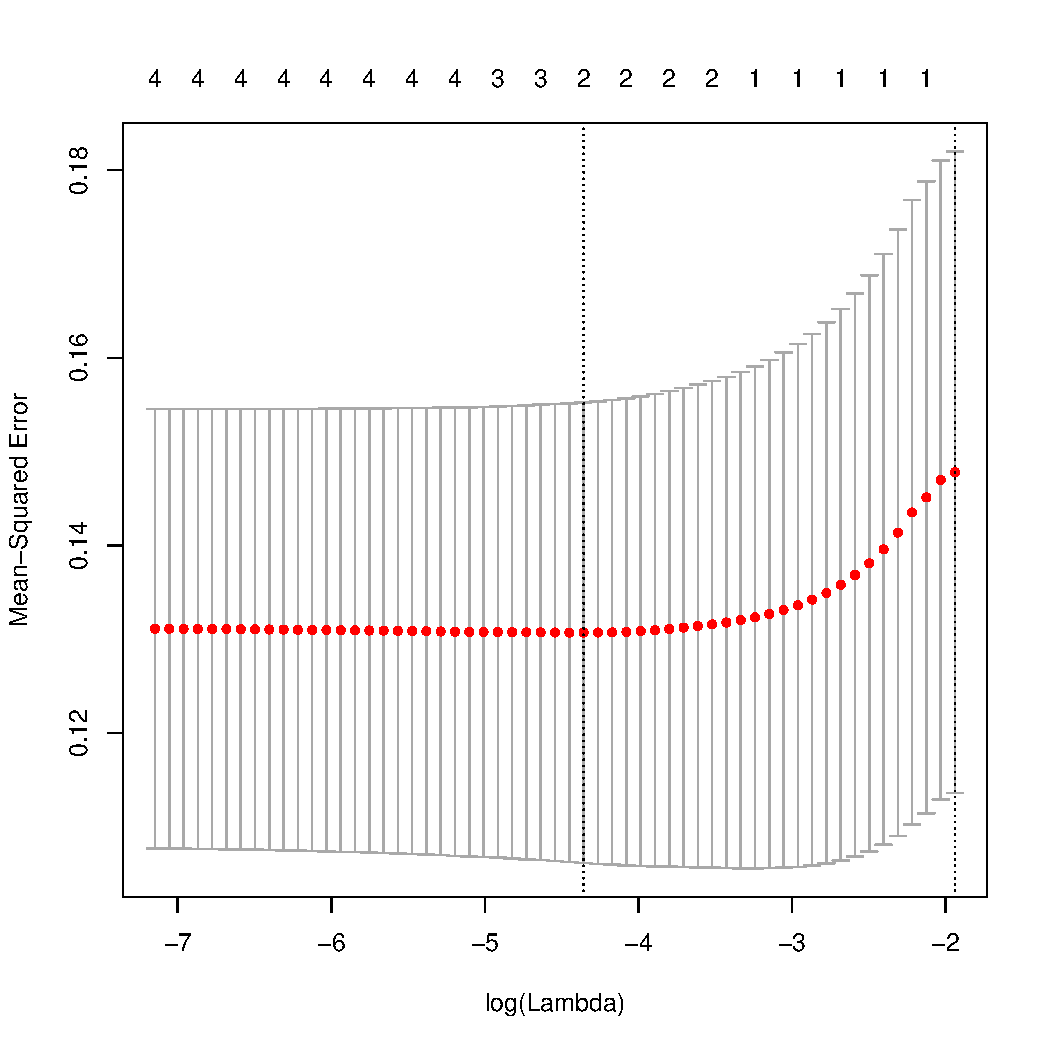
\includegraphics[width=0.40\linewidth]{figure/unnamed-chunk-15-1} 
\begin{kframe}\begin{alltt}
\hlstd{bestlam}\hlkwb{=}\hlstd{cv.out}\hlopt{$}\hlstd{lambda.min}
\hlstd{lasso.pred}\hlkwb{=}\hlkwd{as.numeric}\hlstd{(}\hlkwd{predict}\hlstd{(hep_lasso,}\hlkwc{s}\hlstd{=bestlam ,}\hlkwc{newx}\hlstd{=x[}\hlopt{-}\hlstd{training,],} \hlkwc{type} \hlstd{=} \hlstr{"class"}\hlstd{)[,}\hlnum{1}\hlstd{])}

\hlkwd{mean}\hlstd{(lasso.pred} \hlopt{!=} \hlstd{y[}\hlopt{-}\hlstd{training])}
\end{alltt}
\begin{verbatim}
## [1] 0.28
\end{verbatim}
\begin{alltt}
\hlkwd{table}\hlstd{(lasso.pred, y[}\hlopt{-}\hlstd{training])}
\end{alltt}
\begin{verbatim}
##           
## lasso.pred  1  2
##          2 14 36
\end{verbatim}
\begin{alltt}
\hlstd{out}\hlkwb{=}\hlkwd{glmnet}\hlstd{(x,y,}\hlkwc{alpha}\hlstd{=}\hlnum{1}\hlstd{,}\hlkwc{lambda}\hlstd{=grid)}
\hlstd{lasso.coef}\hlkwb{=}\hlkwd{predict}\hlstd{(out,}\hlkwc{type}\hlstd{=}\hlstr{"coefficients"}\hlstd{,}\hlkwc{s}\hlstd{=bestlam)}
\hlstd{lasso.coef}
\end{alltt}
\begin{verbatim}
## 5 x 1 sparse Matrix of class "dgCMatrix"
##                        1
## (Intercept)  2.217055813
## V2          -0.004685815
## V3           0.137842857
## V5          -0.041284671
## V20         -0.211038872
\end{verbatim}
\end{kframe}
\end{knitrout}

\end{document}
